\documentclass[onecolumn]{article}
\usepackage{graphicx} % Required for inserting images
\usepackage{amsmath}
\usepackage{amsfonts}
\usepackage{pythonhighlight}
\usepackage{datetime}
\usepackage[colorlinks]{hyperref}
\usepackage{titling}
\usepackage{matlab-prettifier}
\usepackage[a4paper, total={6in, 8in}]{geometry}

\makeatletter
\Hy@AtBeginDocument{%
  \def\@pdfborder{0 0 1}% Overrides border definition set with colorlinks=true
  \def\@pdfborderstyle{/S/U/W 1}% Overrides border style set with colorlinks=true
                                % Hyperlink border style will be underline of width 1pt
}
\makeatother

\hypersetup{%
  colorlinks=true,
  linkcolor=blue,
  linkbordercolor=blue,% 
}
\footskip = 1pt
\textheight = 700pt
\setlength{\droptitle}{-10em}

\title{Lab 2 Extra \\ \Large{IN3170 - Microelectronics}}
\author{Andreas Engøy, Erik Røset \& Daniel Tran}
\date{\monthname[\the\month] \the\year}

\begin{document}
\maketitle
\vspace*{50mm}
\tableofcontents

\section{Task 1}

\subsection{Objective}
The objective of this task is to build two CMOS inverter chains of different length and probing before the first and after the last inverter. The purpose of this is to measure and calculate the propagation delay a single inverter without knowing the added capacitance of the scope probe or directly measuring the input capacitance of just one inverter.

\subsection{Equipment}

\begin{table}[h]
    \centering
    \begin{tabular}{|c|c|c|}
        \hline
        \textbf{Component} & \textbf{Model} & \textbf{Quantity} \\
        \hline
        Hex Scmitt-Trigger Inverters & SN74HC1 & 1 \\
        Oscilloscope & HP54622 & 1 \\
        Waveform generator  & HP33120 & 1\\
        Voltage source & HPE3631 & 1 \\
        Breadboard & ~ & 1 \\
        \hline
    \end{tabular}
    \caption{List of components used in task 1.}
    \label{tab:bom}
\end{table}

\clearpage

\subsection{Method}

\begin{figure}[h!]
    \centering
    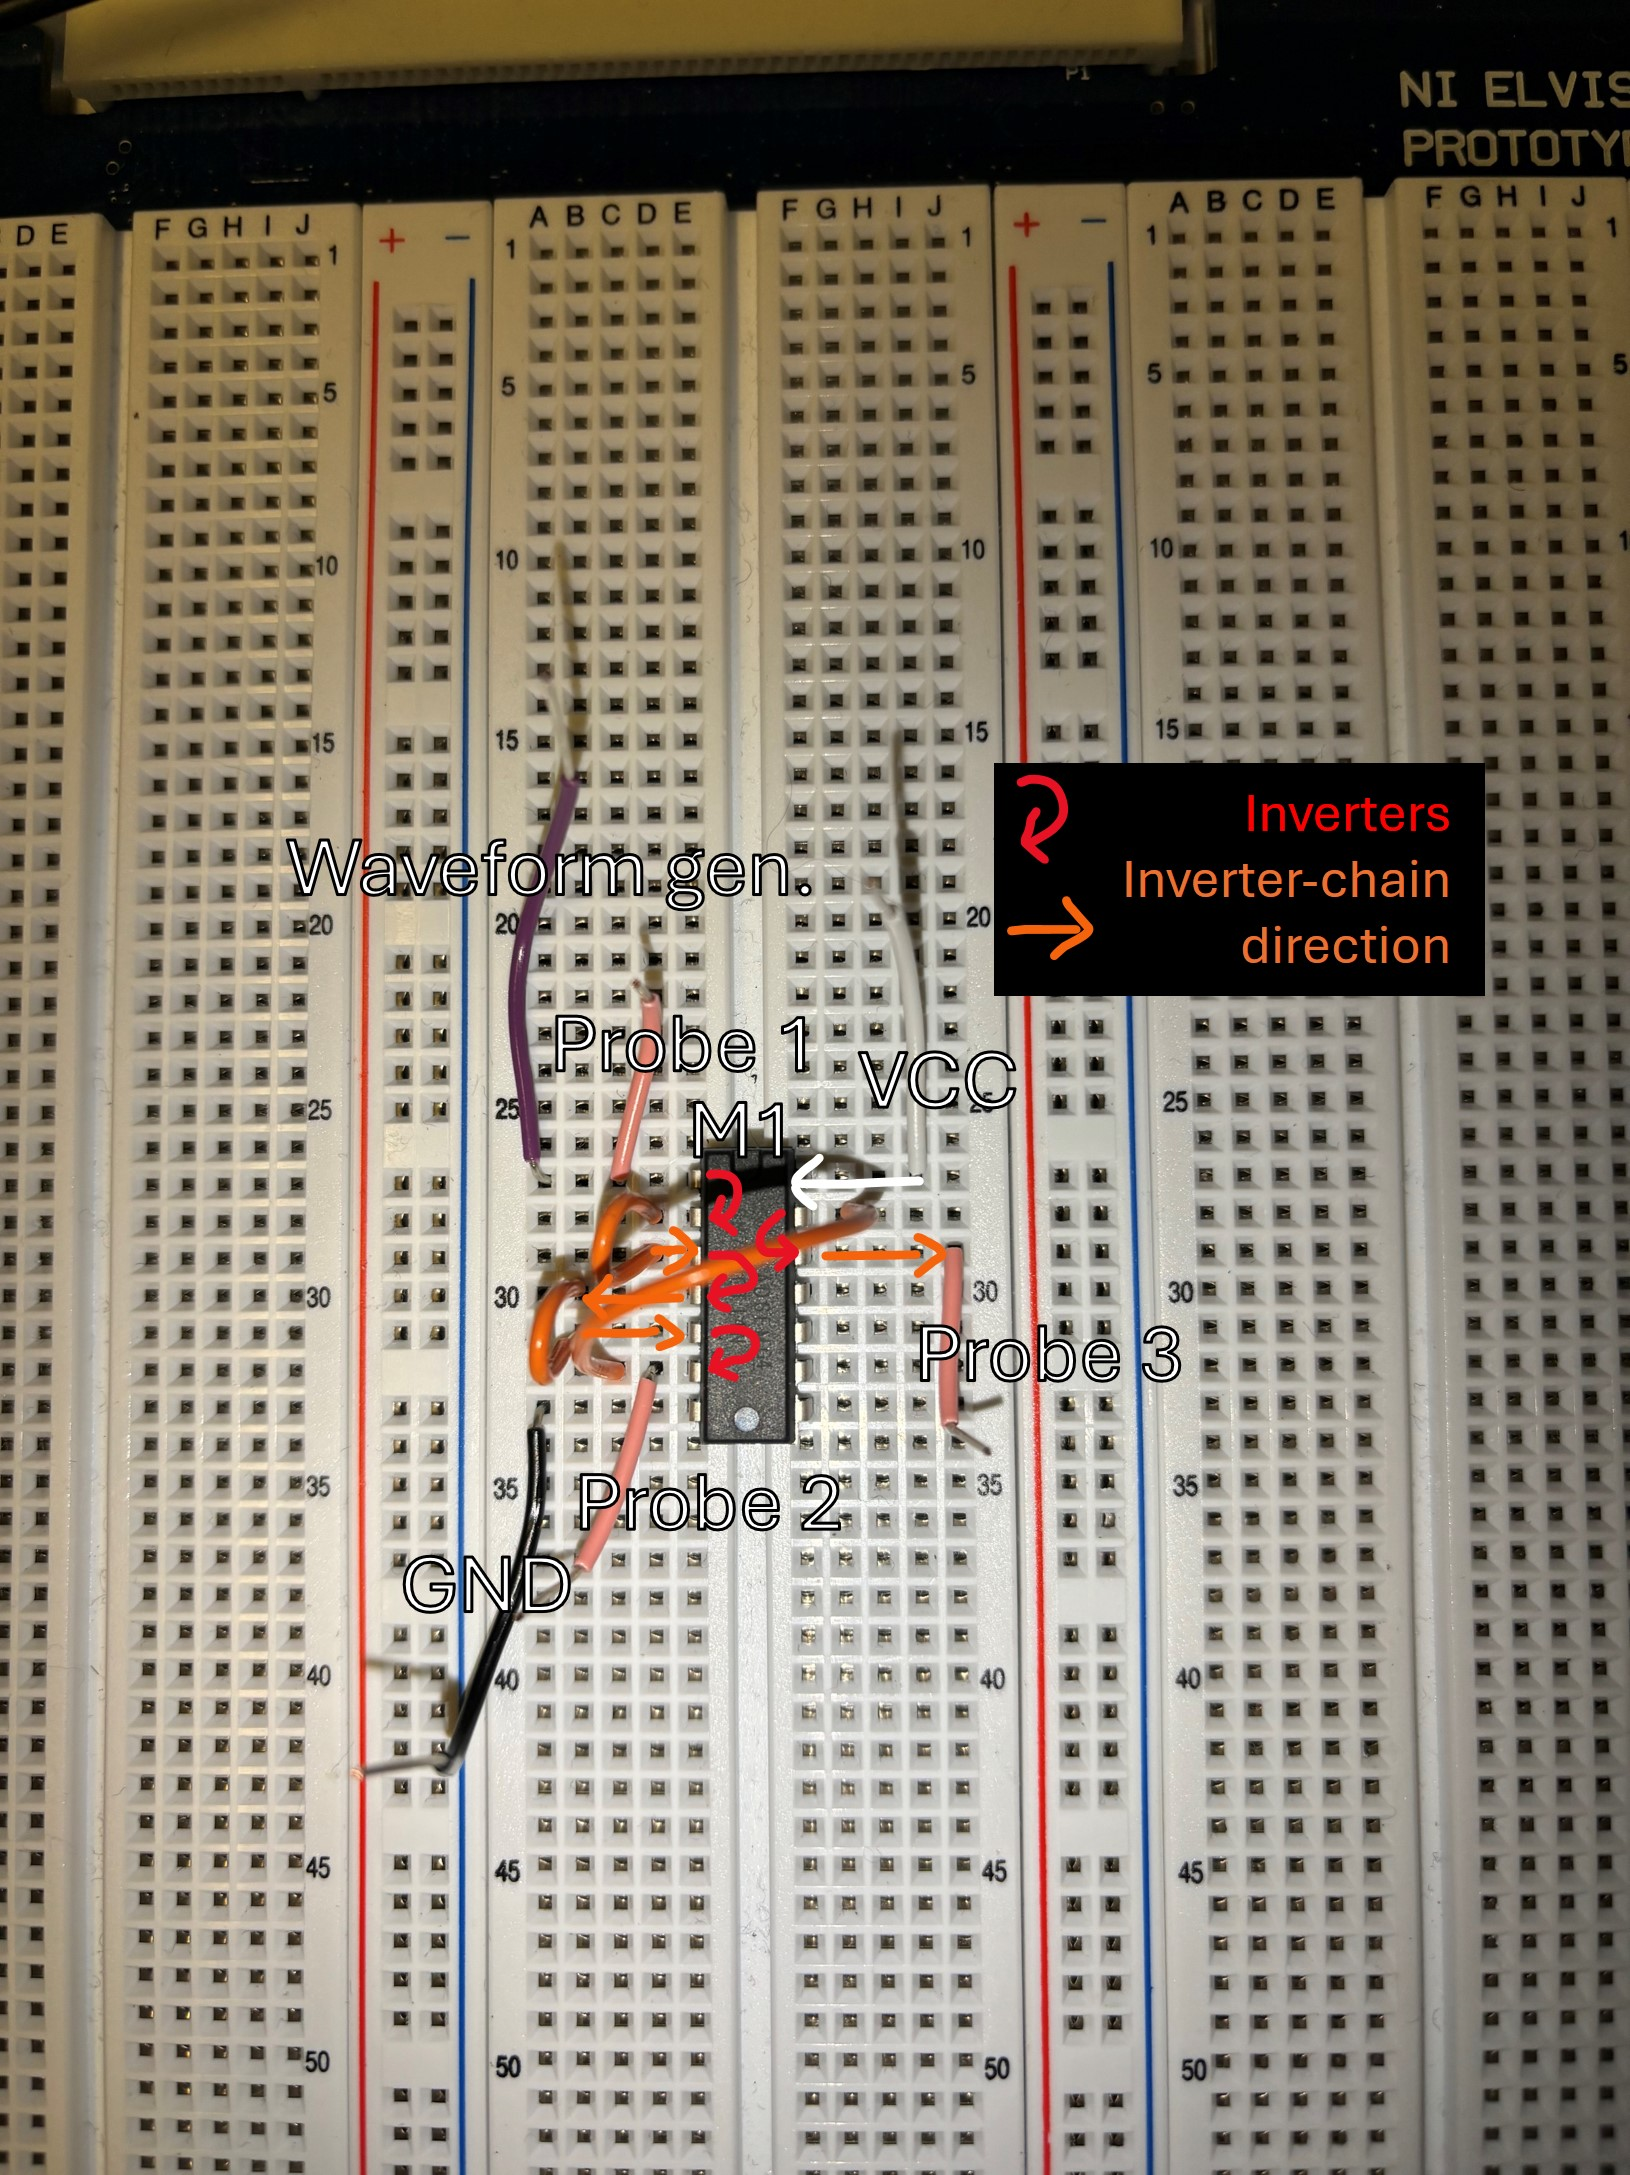
\includegraphics[width=0.5\textwidth]{Circuit_draw.jpg}
    \caption{Picture of the setup for task 1.}  
    \label{fig:circuit}
\end{figure}

\begin{figure}[h!]
    \centering
    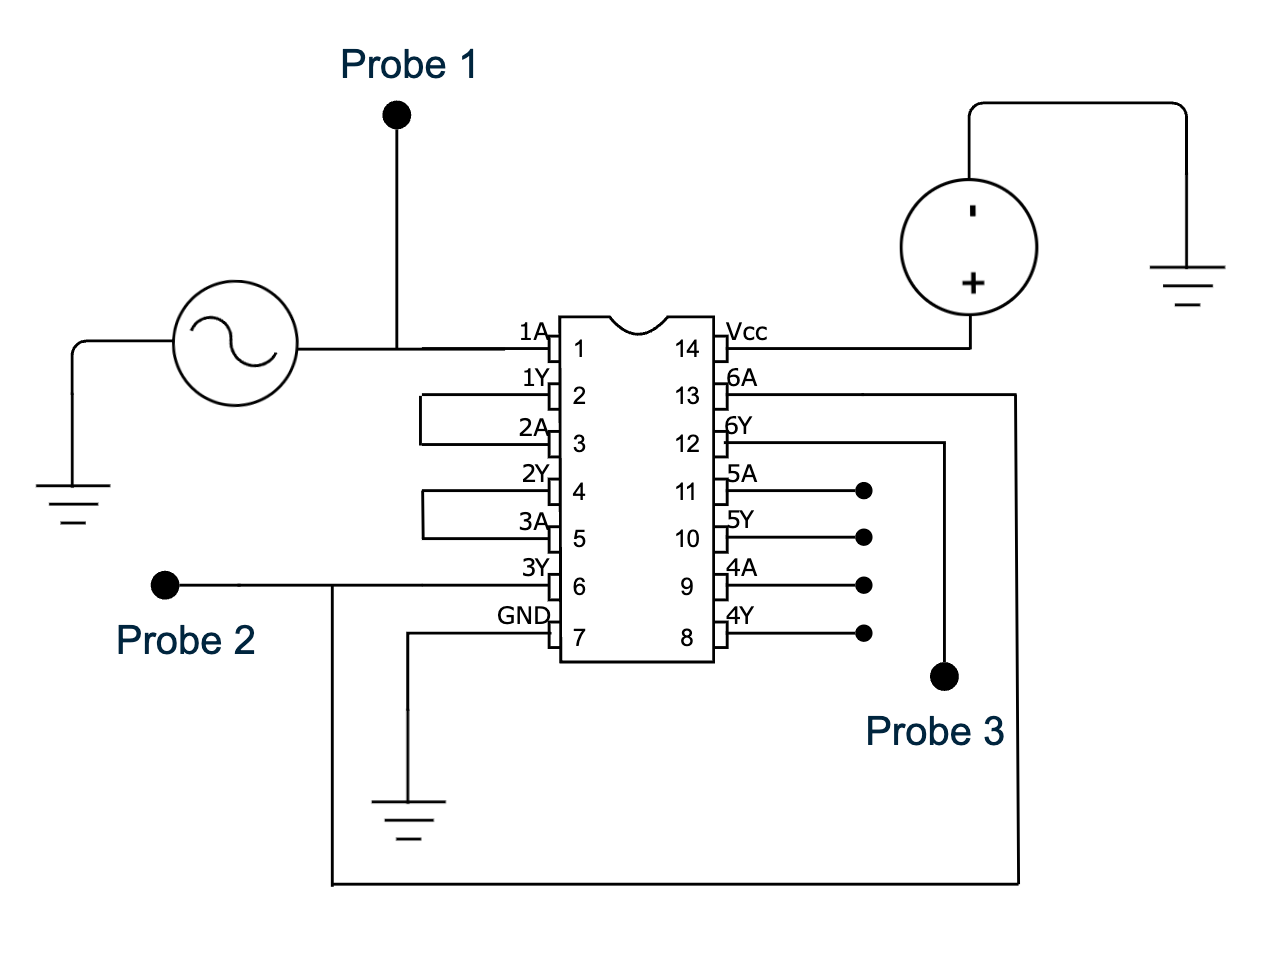
\includegraphics[width=0.5\textwidth]{circuit_schematics.png}
    \caption{Schematic of the setup for task 1.}
    \label{fig:schematic}
\end{figure}


\end{document}